\documentclass[tikz, crop, border = {2pt 2pt 2pt 2pt}]{standalone}

\usepackage{physics}
\usetikzlibrary{decorations.pathreplacing, calligraphy}

\usepackage{concmath-otf}

\begin{document}
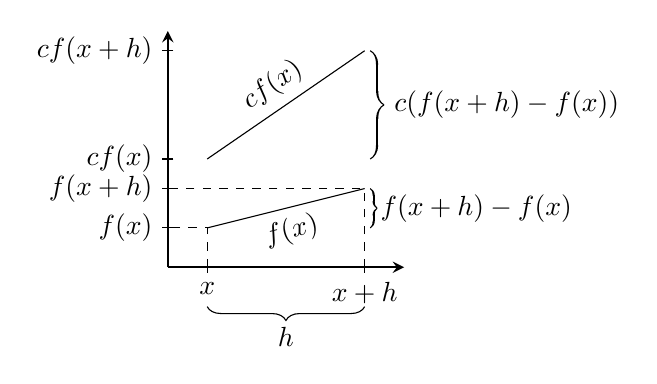
\begin{tikzpicture}
    \draw[thick, -stealth] (0, 0) -- (0, 3);
    \draw[thick, -stealth] (0, 0) -- (3, 0);

    \draw (0.5, 0.5) -- (2.5, 1) node[midway, auto, swap, sloped]{$f(x)$};
    \draw[dashed] (0.5, 0) |- (0, 0.5);
    \draw[dashed] (2.5, 0) |- (0, 1);

    \draw (0.5, 2pt) -- ++ (0, -4pt) node[below]{$x$};
    \draw (2.5, 2pt) -- ++ (0, -4pt) node[below]{$x + h$};
    \draw (2pt, 0.5) -- ++ (-4pt, 0) node[left]{$f(x)$};
    \draw (2pt, 1) -- ++ (-4pt, 0) node[left]{$f(x + h)$};

    \draw (0.5, 1.375) -- (2.5, 2.75) node[midway, auto, sloped]{$cf(x)$};
    \draw (2pt, 1.375) -- ++ (-4pt, 0) node[left]{$cf(x)$};
    \draw (2pt, 2.75) -- ++ (-4pt, 0) node[left]{$cf(x + h)$};

    \draw[decorate, decoration = {brace, amplitude = 5pt, raise = 2pt, calligraphic brace}, thick] (2.5, 2.75) -- (2.5, 1.375) node[midway, right = 7pt]{$c(f(x + h) - f(x))$};
    \draw[decorate, decoration = {brace, raise = 2pt, calligraphic brace}, thick] (2.5, 1) -- (2.5, 0.5) node[midway, right = 2pt]{$f(x + h) - f(x)$};
    \draw[decorate, decoration = {brace, amplitude = 5pt, mirror}] (0.5, -0.5) -- ++ (2, 0) node[midway, below = 4pt]{$h$};
\end{tikzpicture}
\end{document}